\chapter{Voice Assistance}

We spend so much time using devices that have integrated voice assistants that we usually forget how incredibly fast they have
evolved. Nowadays, they can recognize thousands of words and expressions really fast, and they are even capable to imitate
emotions. What is more, they fit in a pocket. But the reality was totally different just a couple of decades ago. From the IBM
Shoebox to Siri, in this chapter I will explore the fundamentals of voice assistance.

\section{What is Voice Assistance?}
Voice assistance is the result of another form of interaction between humans and computers.\cite{botsocietyVUI} The Voice User
Interface (VUI), which has the voice assistants as a result, allows a user to interact with computer or mobile or other electronic 
devices through speech or voice commands. Thus, VUI is an interface of any speech recognition applications.

Therefore, a voice assistance, also known as virtual assistant, is an application program that understands natural language voice 
commands and can perform tasks or services for an individual. Its expansion has been truly remarkable in the last few years, to the
point that we can see devices that exclusively work as virtual assistants, with integration with many other services. Its real usefulness
in society, though, remains to be seen, as this field is commonly viewed with skepticism and mistrust, and the fact of talking to a 
machine as if it were another human being remains an obstacle to overcome.

As I mentioned, voice assistants are now present in plenty of platforms:
\begin{itemize}
	\item \textbf{Smart speakers:} Google Home (Fig. \ref{fig:google-home}), Apple HomePod, Amazon Echo, Movistar Home.
	\item \textbf{Mobile operating systems:} Siri on iOS, Google Assistant on Android, Bixby on Samsung phones.
	\item \textbf{Desktop operating systems:} Siri on macOS and Cortana on Windows 10.
	\item \textbf{Smartwatches}: Apple Watch, Google Wear OS.
	\item \textbf{Cars:} Apple CarPlay, Android Auto. 
	\item \textbf{Televisions:} Siri on Apple TV (Fig. \ref{fig:apple-tv}) and the voice assistant in Samsung Smart TVs.
	\item \textbf{Inside mobile apps:} EVO Assistant in the mobile application of the Spanish bank EVO.
\end{itemize}

\begin{figure}
	\centering
	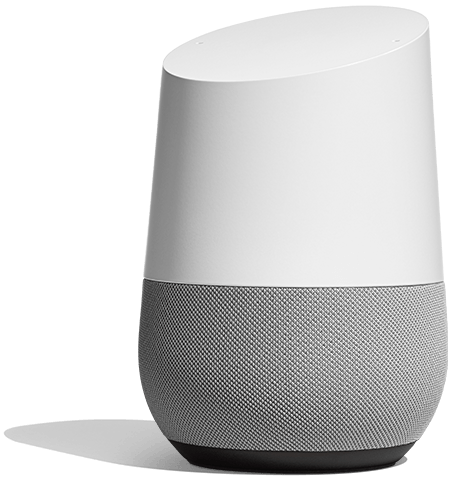
\includegraphics[width=0.5\textwidth]{images/Chapter_03/google-home.png}
	\caption{Google Home, a smart speaker integrated with the Google Assistant}
	\label{fig:google-home}
\end{figure}

\begin{figure}
	\centering
	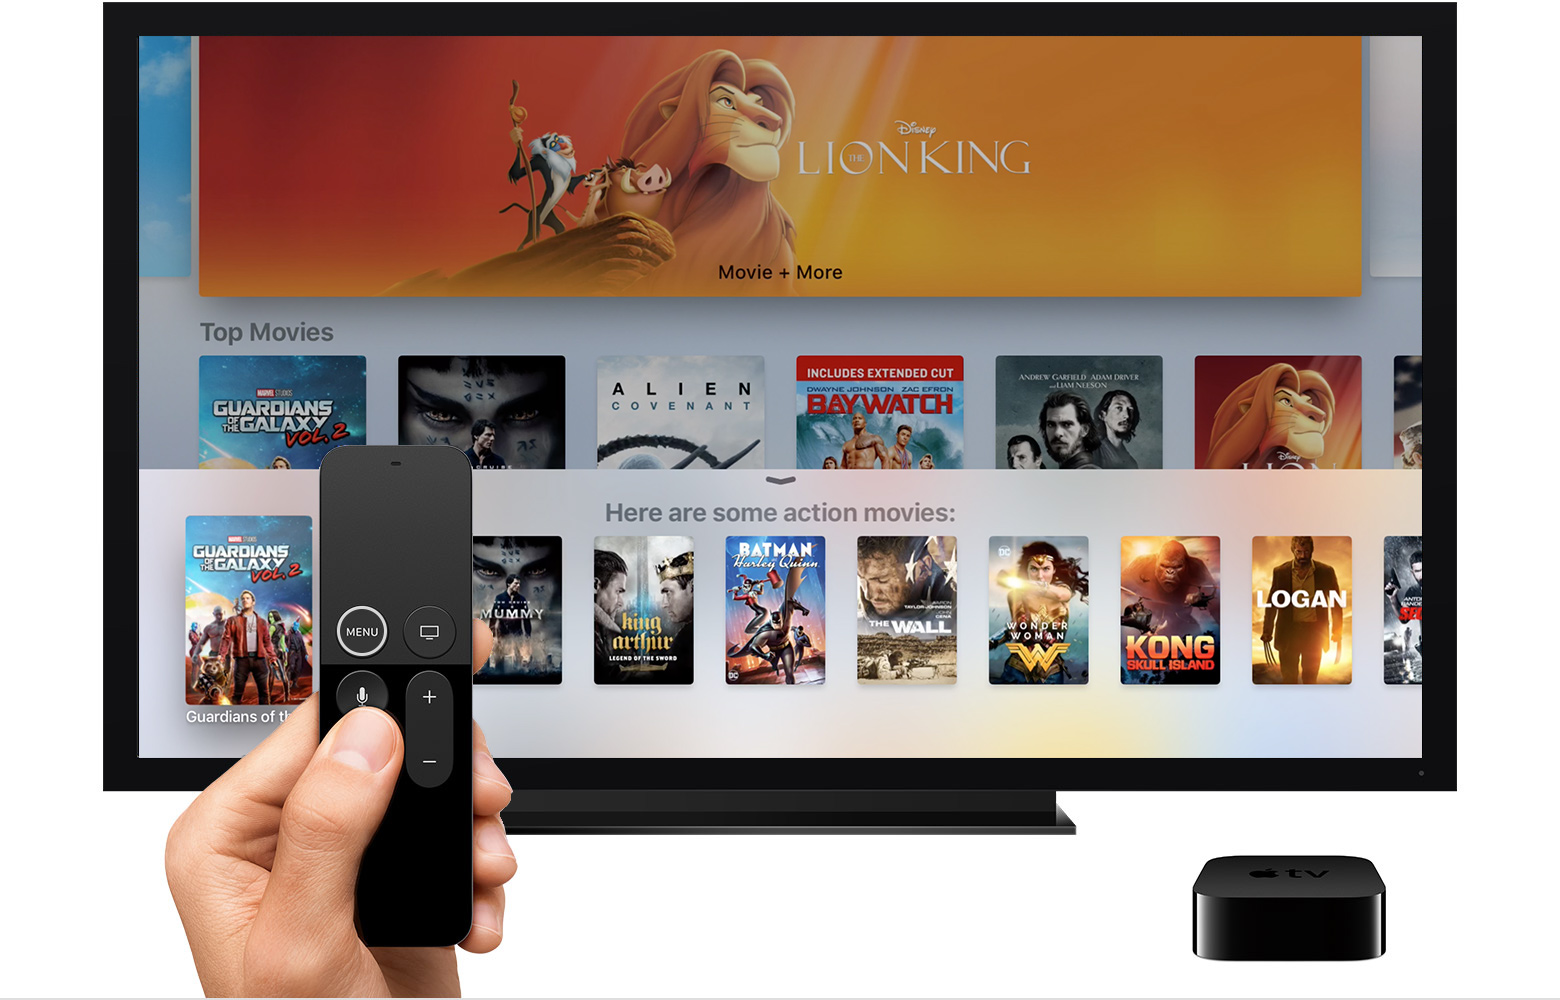
\includegraphics[width=0.9\textwidth]{images/Chapter_03/apple-tv.jpg}
	\caption{Apple TV and the Siri Remote, which has a microphone to interact with the assistant}
	\label{fig:apple-tv}
\end{figure}

The history of voice assistance goes back to 1961, when IBM introduced the IBM Shoebox.\cite{voicebotTimeline} 
This was a very innovative product at that moment. Although it was not suitable for commercial use, it did mark the 
beginning of a revolution, the fruits of which we can now see. 

The Shoebox was capable of recognizing 16 spoken words, including ten digits from 0 through 9. When a number and 
command words such as \textit{plus}, \textit{minus} and \textit{total} were spoken, Shoebox instructed an adding machine 
to calculate and print answers to simple arithmetic problems. It classified the electrical impulses generated from a microphone
according to various types of sounds and activated the attached adding machine through a relay system.\cite{ibmArchivesShoebox}

Later on, there were more attempts from the research field, as the HARPY Speech Recognition System from the Carnegie
Mellon University, in 1976.\cite{lowerre76} Is could recognize about 1000 words.

Nevertheless, it was not until 1990 that the first speech recognition for consumers appeared: the Dragon Dictate. Seven years
later, the same company presented the Dragon NaturallySpeaking, which introduced continuous speech recognition as a novelty.
They led the way with competent voice recognition and transcription. This field attracted the attention from big companies of that 
time, and Microsoft began working on their own assistant: Clippy, in the Microsoft Office suite. In spite of the fact that this was 
not a voice assistant exactly, it showed how natural language could be interpreted and used in order to allow the human-computer
interaction. It was quite unpopular and Microsoft decided to end it on 2001, but its impact was huge for the assistants that followed
it. A bit before Windows XP, Microsoft introduced the speech recognition feature in their Office XP suite.

With the launch of Siri in 2014, Apple marked the modern era of voice assistants. For the first time, people could fit a full functional
voice assistant in their pocket. And most importantly, Siri reached a wide audience and began to popularize this technology.
Siri was able to make searches on Internet and reproduce the results, to set reminders and events in the calendar or to call any
contact by its name, between many others. In addition, it included a layer of \textit{natural interaction} with the user, being able to 
respond to any other phrase as any other human would (even to sentences that were not commands, like \textit{How do you feel 
today?} or \textit{Tell me a joke}).

Google, with Google Now, and then Microsoft and Amazon, with Cortana and Alexa respectively, followed this trend, even improving
on what Siri failed, and in the case of Microsoft, making a voice assistant available on PCs as well. Then, in 2014, Amazon introduced
Echo, the first smart speaker of all time. It was just the beginning of what we now call the \textit{Smart Speaker Revolution}.\cite{voicebotTimeline}

After the Echo, Apple and Google followed with the HomePod and Home, respectively. In fact, Google Home has been recently
launched in Spain, and the HomePod is not available yet, as an example of how recent this technology is. Its number of users is 
expected to continue to grow, and even faster than it has already done.\cite{statistaDigitalAssistants}

\begin{figure}
	\centering
	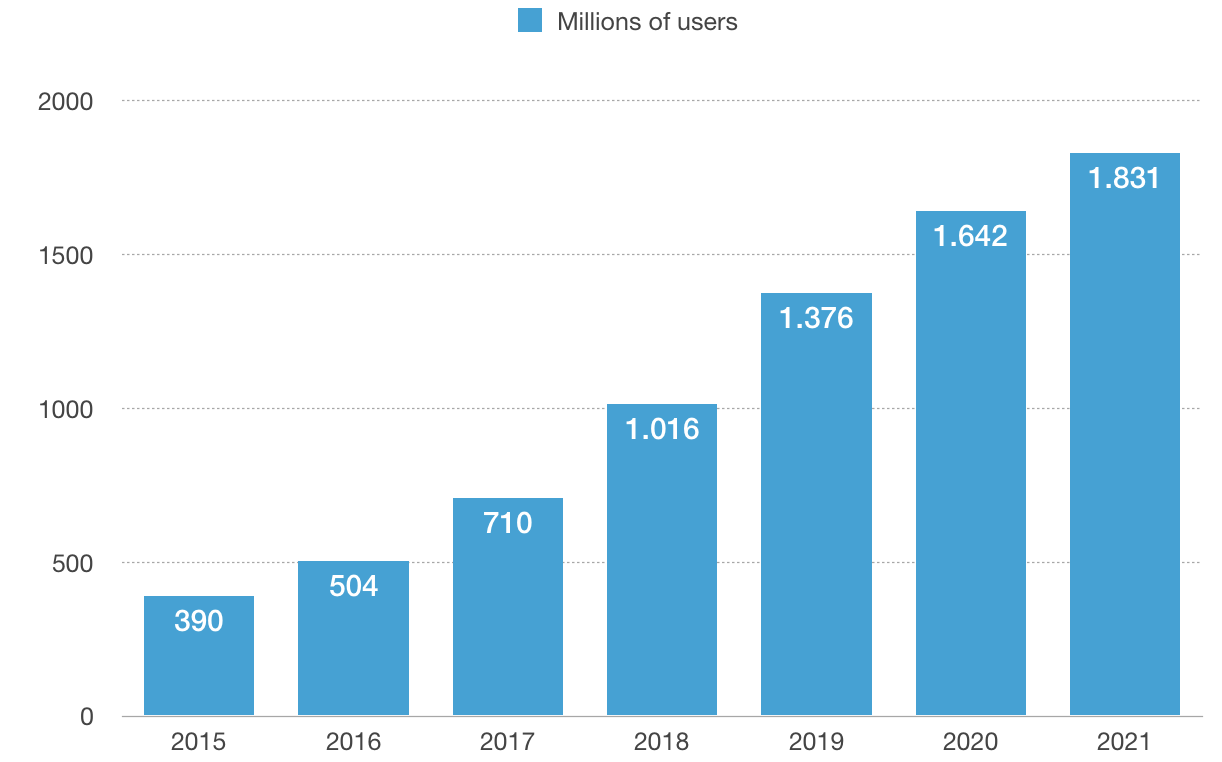
\includegraphics[width=0.9\textwidth]{images/Chapter_03/voice-assistants-usage.png}
	\caption{Estimated number of users of virtual assistants worldwide, from 2015 to 2021\cite{statistaDigitalAssistants}}
	\label{fig:voice-assistants-usage}
\end{figure}

\section{Services Voice Assistants Provide}
The range of services provided by voice assistants is constantly becoming bigger, as they are a booming technology that is constantly
receiving new updates. The following are shared by most of the virtual assistants currently:
\begin{itemize}
	\item Provide information, such as weather forecast, routes to any point in a map or general knowledge.
	\item Manage components in a Home Automation environment.
	\item Interact with media content, such as music and video (which is commonly integrated with streaming services, like Netfix or 
	Apple Music).
	\item Make phone calls and send instant messages.
	\item Manage the personal agenda.
	\item Provide accessibility indications.
	\item In call centers, they complement or replace the customer service by humans.
\end{itemize}

We are nowadays in the first stages of this new technology, that combines artificial intelligence, machine learning, voice recognition 
and human-computer interaction. Google is the company that apparently has done the biggest advancements and, in fact, they have 
recently introduced Google Duplex, a technology capable of almost perfectly simulating a human speech, which can be used for a wide
range of purposes, such as ordering food or making an appointment with a hairdresser. This would be a new service to include in 
the previous list.

They are also providing very useful tools to developers and makers, like the Cloud Speech-To-Text API. I will come back to this 
technology in the following chapters, as it will be an essential part to achieve my objective, the creation of a voice-driven home 
automation controller, a service that can also be seen in the previous list.

